\section{积分的应用}

\begin{problem}{平面曲线弧长的计算}{Arc-Length-Of-Plane-Curves}
    求下列曲线弧的弧长：
    \begin{enumerate}
        \item 抛物线 $y = x^2$ 从 $x = -a$ 到 $x = a$ 之间的弧；
        \item 星形线 $\begin{dcases} x = a\cos^3 t, \\ y = a\sin^3 t \end{dcases} (0 \leqslant t < 2\uppi)$，$a > 0$ 是常数；
        \item Archimedes 螺线 $r = a\theta$ ($0 \leqslant \theta \leqslant 2\uppi$)．
    \end{enumerate}
\end{problem}

\begin{solution}
    \ansitem{1}

    由弧长微分公式 $\d s = \sqrt{1 + (y')^2}\d x = \sqrt{1 + 4x^2}\d x$，利用对称性：
    \begin{equation}
        s = \int_{-a}^a \sqrt{1 + 4x^2}\d x = 2\int_0^a \sqrt{1 + 4x^2}\d x.
    \end{equation}
    利用标准不定积分公式 $\int \sqrt{1 + 4x^2}\d x = \frac{x}{2}\sqrt{1 + 4x^2} + \frac{1}{4}\ln\bigl(2x + \sqrt{1 + 4x^2}\bigr)$，代入上下限得
    \begin{equation}
        s = 2\left[ \frac{a}{2}\sqrt{1 + 4a^2} + \frac{1}{4}\ln\bigl(2a + \sqrt{1 + 4a^2}\bigr) \right] = a\sqrt{1 + 4a^2} + \frac{1}{2}\ln\bigl(2a + \sqrt{1 + 4a^2}\bigr).
    \end{equation}
    \begin{equation}
        \boxed{s = a\sqrt{1 + 4a^2} + \frac{1}{2}\ln\bigl(2a + \sqrt{1 + 4a^2}\bigr).}
    \end{equation}

    \ansitem{2}

    计算参数导数：
    \begin{equation}
        x'(t) = -3a\cos^2 t \sin t, \qquad y'(t) = 3a\sin^2 t \cos t.
    \end{equation}
    弧长微元为
    \begin{equation}
        \d s = \sqrt{[x'(t)]^2 + [y'(t)]^2}\d t = 3a|\sin t \cos t|\d t.
    \end{equation}
    由星形线在四个象限的对称性：
    \begin{equation}
        s = 4 \int_0^{\frac{\uppi}{2}} 3a\sin t \cos t \d t = 12a \left[ \frac{\sin^2 t}{2} \right]_0^{\frac{\uppi}{2}} = 6a.
    \end{equation}
    \begin{equation}
        \boxed{s = 6a.}
    \end{equation}

    \ansitem{3}

    在极坐标系下，弧长微元为 $\d s = \sqrt{r^2 + (r')^2}\d\theta = \sqrt{a^2\theta^2 + a^2}\d\theta = a\sqrt{1 + \theta^2}\d\theta$：
    \begin{equation}
        \begin{aligned}
            s & = a \int_0^{2\uppi} \sqrt{1 + \theta^2}\d\theta                                                                            \\
              & = a \left[ \frac{\theta}{2}\sqrt{1 + \theta^2} + \frac{1}{2}\ln\bigl(\theta + \sqrt{1 + \theta^2}\bigr) \right]_0^{2\uppi} \\
              & = a\uppi\sqrt{1 + 4\uppi^2} + \frac{a}{2}\ln\bigl(2\uppi + \sqrt{1 + 4\uppi^2}\bigr).
        \end{aligned}
    \end{equation}
    \begin{equation}
        \boxed{s = a\uppi\sqrt{1 + 4\uppi^2} + \frac{a}{2}\ln\bigl(2\uppi + \sqrt{1 + 4\uppi^2}\bigr).}
    \end{equation}
\end{solution}

\begin{problem}{平面图形面积的计算}{Area-Of-Plane-Regions}
    计算下面的曲线所围成的平面图形的面积：
    \begin{enumerate}
        \item 双纽线 $r^2 = a^2 \cos 2\theta$（$\theta \in \left[-\frac{\uppi}{4}, \frac{\uppi}{4}\right] \cup \left[\frac{3\uppi}{4}, \frac{5\uppi}{4}\right]$，$a$ 为正常数）；
        \item $\begin{dcases} x = t - \sin t, \\ y = 1 - \cos t \end{dcases} (0 \leqslant t \leqslant 2\uppi)$ 及 $x$ 轴；
        \item $y = \e^x$、$y = \e^{-x}$ 及 $x = 1$．
    \end{enumerate}
\end{problem}

\begin{solution}
    \ansitem{1}

    双纽线包含关于原点对称的左右两瓣，利用对称性计算总面积：
    \begin{equation}
        S = 2 \cdot \frac{1}{2}\int_{-\frac{\uppi}{4}}^{\frac{\uppi}{4}} r^2 \d\theta = \int_{-\frac{\uppi}{4}}^{\frac{\uppi}{4}} a^2 \cos 2\theta \d\theta = a^2 \left[ \frac{\sin 2\theta}{2} \right]_{-\frac{\uppi}{4}}^{\frac{\uppi}{4}} = a^2.
    \end{equation}
    \begin{equation}
        \boxed{S = a^2.}
    \end{equation}

    \ansitem{2}

    曲线为一拱摆线，以 $t$ 为参数由定积分公式计算：
    \begin{equation}
        \begin{aligned}
            S & = \int_0^{2\uppi} y(t) x'(t)\d t = \int_0^{2\uppi} (1 - \cos t)^2 \d t        \\
              & = \int_0^{2\uppi} (1 - 2\cos t + \cos^2 t)\d t = 2\uppi - 0 + \uppi = 3\uppi.
        \end{aligned}
    \end{equation}
    \begin{equation}
        \boxed{S = 3\uppi.}
    \end{equation}

    \ansitem{3}

    两曲线 $y = \e^x$ 与 $y = \e^{-x}$ 在 $x = 0$ 处相交，当 $x \in [0, 1]$ 时恒有 $\e^x \geqslant \e^{-x}$．

    \begin{center}
        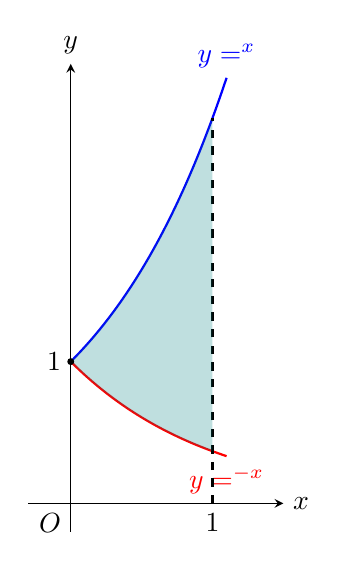
\begin{tikzpicture}[>=stealth, scale=1.8]
            \draw[->] (-0.3, 0) -- (1.5, 0) node[right] {$x$};
            \draw[->] (0, -0.2) -- (0, 3.1) node[above] {$y$};
            \node[below left] at (0, 0) {$O$};

            \draw[domain=0:1.1, samples=80, smooth, thick, blue] plot (\x, {exp(\x)}) node[above] {$y = \e^x$};
            \draw[domain=0:1.1, samples=80, smooth, thick, red] plot (\x, {exp(-\x)}) node[below] {$y = \e^{-x}$};
            \draw[dashed, thick] (1, 0) node[below] {$1$} -- (1, {exp(1)});

            \fill[teal, opacity=0.25, domain=0:1, samples=80]
            plot (\x, {exp(\x)}) -- (1, {exp(-1)}) -- plot[domain=1:0] (\x, {exp(-\x)}) -- cycle;
            \fill (0,1) circle (0.7pt) node[left] {$1$};
        \end{tikzpicture}
    \end{center}

    平面图形的面积为
    \begin{equation}
        S = \int_0^1 (\e^x - \e^{-x})\d x = [\e^x + \e^{-x}]_0^1 = \e + \e^{-1} - 2.
    \end{equation}
    \begin{equation}
        \boxed{S = \e + \frac{1}{\e} - 2.}
    \end{equation}
\end{solution}

\begin{problem}{旋转体体积的计算}{Volume-Of-Solids-Of-Revolution}
    计算下列旋转体的体积：
    \begin{enumerate}
        \item $y = \sin x$ ($0 \leqslant x < \uppi$) 与 $x$ 轴围成的图形分别绕 $x$ 轴及 $y$ 轴旋转一周；
        \item $y = \e^{x^2}$ ($0 \leqslant x \leqslant 1$) 与 $x$ 轴围成的图形绕 $y$ 轴旋转一周；
        \item $\begin{dcases} x = t - \sin t, \\ y = 1 - \cos t \end{dcases} (0 \leqslant t \leqslant 2\uppi)$ 与 $x$ 轴围成的图形绕 $x$ 轴旋转一周．
    \end{enumerate}
\end{problem}

\begin{solution}
    \ansitem{1}

    绕 $x$ 轴旋转所得旋转体体积：
    \begin{equation}
        V_x = \uppi \int_0^{\uppi} \sin^2 x \d x = \uppi \int_0^{\uppi} \frac{1 - \cos 2x}{2}\d x = \frac{\uppi^2}{2}.
    \end{equation}
    绕 $y$ 轴旋转，利用圆柱壳法：
    \begin{equation}
        V_y = 2\uppi \int_0^{\uppi} x \sin x \d x = 2\uppi [\sin x - x\cos x]_0^{\uppi} = 2\uppi^2.
    \end{equation}
    \begin{equation}
        \boxed{V_x = \frac{\uppi^2}{2}, \qquad V_y = 2\uppi^2.}
    \end{equation}

    \ansitem{2}

    利用圆柱壳法（柱壳面积元为 $2\uppi x y \d x$）：
    \begin{equation}
        V_y = 2\uppi \int_0^1 x \e^{x^2}\d x = \uppi \int_0^1 \e^{x^2}\d(x^2) = \uppi [\e^{x^2}]_0^1 = \uppi(\e - 1).
    \end{equation}
    \begin{equation}
        \boxed{V_y = \uppi(\e - 1).}
    \end{equation}

    \ansitem{3}

    利用参数形式的旋转体体积微元 $\d V_x = \uppi y^2 \d x = \uppi y^2(t) x'(t)\d t$：
    \begin{equation}
        \begin{aligned}
            V_x & = \uppi \int_0^{2\uppi} (1 - \cos t)^3 \d t                      \\
                & = \uppi \int_0^{2\uppi} (1 - 3\cos t + 3\cos^2 t - \cos^3 t)\d t \\
                & = \uppi (2\uppi - 0 + 3\uppi - 0) = 5\uppi^2.
        \end{aligned}
    \end{equation}
    \begin{equation}
        \boxed{V_x = 5\uppi^2.}
    \end{equation}
\end{solution}

\begin{problem}{球缺体积公式的推导}{Volume-Of-Spherical-Cap}
    求证：以 $R$ 为半径，高为 $h$ 的球缺的体积为 $\uppi h^2 \left(R - \frac{h}{3}\right)$．
\end{problem}

\begin{myproof}
    建立直角坐标系，设球面方程为 $x^2 + y^2 + z^2 = R^2$．球缺对应高度区间为 $z \in [R - h, R]$．

    \begin{center}
        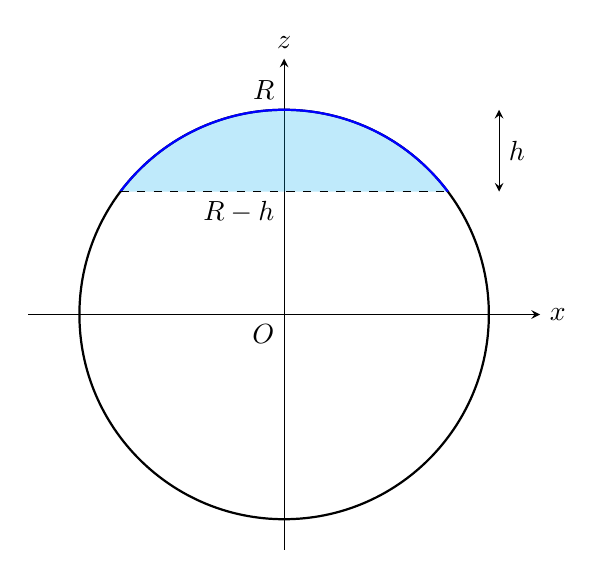
\begin{tikzpicture}[>=stealth, scale=1.3]
            \draw[->] (-2.5, 0) -- (2.5, 0) node[right] {$x$};
            \draw[->] (0, -2.3) -- (0, 2.5) node[above] {$z$};
            \node[below left] at (0, 0) {$O$};

            \draw[thick] (0,0) circle (2);

            % Cap region: R = 2, h = 0.8 => z from 1.2 to 2.0
            % sqrt(4 - 1.2^2) = sqrt(2.56) = 1.6
            \fill[cyan, opacity=0.25] (-1.6, 1.2) arc (143.13:36.87:2) -- cycle;
            \draw[thick, blue] (-1.6, 1.2) arc (143.13:36.87:2);
            \draw[dashed] (-1.6, 1.2) -- (1.6, 1.2);

            \draw[<->] (2.1, 1.2) -- (2.1, 2) node[midway, right] {$h$};
            \draw (0, 1.2) node[below left] {$R - h$};
            \draw (0, 2) node[above left] {$R$};
        \end{tikzpicture}
    \end{center}

    在高度 $z$ 处垂直于 $z$ 轴的横截面为圆形，其半径满足 $r(z) = \sqrt{R^2 - z^2}$，截面积为
    \begin{equation}
        A(z) = \uppi (R^2 - z^2).
    \end{equation}
    对横截面积沿高度积分：
    \begin{equation}
        V = \int_{R-h}^R \uppi (R^2 - z^2)\d z.
    \end{equation}
    作变量代换 $u = R - z$（$u \in [0, h]$），$\d z = -\d u$，$R^2 - z^2 = 2Ru - u^2$：
    \begin{equation}
        V = \uppi \int_0^h (2Ru - u^2)\d u = \uppi \left[ Ru^2 - \frac{u^3}{3} \right]_0^h = \uppi h^2 \left( R - \frac{h}{3} \right).
    \end{equation}
    命题得证．
\end{myproof}

\begin{problem}{旋转曲面的侧面积计算}{Lateral-Surface-Area-Of-Revolution}
    求下列曲线段旋转一周后所得立体的侧面积：
    \begin{enumerate}
        \item $x^2 + y^2 = r^2$ 绕 $x$ 轴，其中常数 $r > 0$；
        \item $\frac{x^2}{a^2} + \frac{y^2}{b^2} = 1$ 绕 $y$ 轴，这里 $a > b > 0$；
        \item $y = a\cosh x$ ($0 \leqslant x \leqslant a$) 绕 $x$ 轴；
        \item $r = a(1 + \cos\theta)$ 绕极轴，$a > 0$．
    \end{enumerate}
\end{problem}

\begin{solution}
    \ansitem{1}

    上半圆周方程为 $y = \sqrt{r^2 - x^2}$（$x \in [-r, r]$），弧长微元 $\d s = \frac{r}{\sqrt{r^2 - x^2}}\d x$：
    \begin{equation}
        S = 2\uppi \int_{-r}^r y \d s = 2\uppi \int_{-r}^r \sqrt{r^2 - x^2} \cdot \frac{r}{\sqrt{r^2 - x^2}}\d x = 2\uppi r \int_{-r}^r \d x = 4\uppi r^2.
    \end{equation}
    \begin{equation}
        \boxed{S = 4\uppi r^2.}
    \end{equation}

    \ansitem{2}

    椭圆参数方程为 $x = a\cos t$，$y = b\sin t$（$t \in \left[-\frac{\uppi}{2}, \frac{\uppi}{2}\right]$）．记离心率 $e = \frac{\sqrt{a^2 - b^2}}{a}$．

    绕 $y$ 轴旋转的面积微元 $\d S = 2\uppi x \d s = 2\uppi (a\cos t)\sqrt{a^2\sin^2 t + b^2\cos^2 t}\d t$：
    \begin{equation}
        \begin{aligned}
            S & = 4\uppi a \int_0^{\frac{\uppi}{2}} \cos t \sqrt{b^2 + a^2 e^2 \sin^2 t}\d t                                            \\
              & = \frac{4\uppi}{e} \int_0^{ae} \sqrt{b^2 + u^2}\d u                                                                     \\
              & = \frac{4\uppi}{e} \left[ \frac{u}{2}\sqrt{b^2 + u^2} + \frac{b^2}{2}\ln\bigl(u + \sqrt{b^2 + u^2}\bigr) \right]_0^{ae} \\
              & = 2\uppi a^2 + \frac{2\uppi b^2}{e}\ln\frac{a(1 + e)}{b}.
        \end{aligned}
    \end{equation}
    \begin{equation}
        \boxed{S = 2\uppi a^2 + \frac{2\uppi b^2}{e}\ln\frac{a(1 + e)}{b}.}
    \end{equation}

    \ansitem{3}

    由 $y = a\cosh x$，导数 $y' = a\sinh x$，弧长微元 $\d s = \sqrt{1 + a^2\sinh^2 x}\d x$：
    \begin{equation}
        S = 2\uppi \int_0^a y \d s = 2\uppi \int_0^a a\cosh x \sqrt{1 + a^2\sinh^2 x}\d x.
    \end{equation}
    令 $u = a\sinh x$，则 $\d u = a\cosh x \d x$：
    \begin{equation}
        \begin{aligned}
            S & = 2\uppi \int_0^{a\sinh a} \sqrt{1 + u^2}\d u                                                      \\
              & = \uppi \left[ u\sqrt{1 + u^2} + \ln\bigl(u + \sqrt{1 + u^2}\bigr) \right]_0^{a\sinh a}            \\
              & = \uppi a\sinh a \sqrt{1 + a^2\sinh^2 a} + \uppi\ln\bigl(a\sinh a + \sqrt{1 + a^2\sinh^2 a}\bigr).
        \end{aligned}
    \end{equation}
    \begin{equation}
        \boxed{S = \uppi a\sinh a \sqrt{1 + a^2\sinh^2 a} + \uppi\ln\bigl(a\sinh a + \sqrt{1 + a^2\sinh^2 a}\bigr).}
    \end{equation}

    \ansitem{4}

    极坐标下极轴即 $x$ 轴，$y = r\sin\theta = 4a\sin\frac{\theta}{2}\cos^3\frac{\theta}{2}$，$\d s = 2a\cos\frac{\theta}{2}\d\theta$（$\theta \in [0, \uppi]$）：
    \begin{equation}
        \begin{aligned}
            S & = 2\uppi \int_0^{\uppi} y(\theta)\d s = 16\uppi a^2 \int_0^{\uppi} \cos^4\frac{\theta}{2}\sin\frac{\theta}{2}\d\theta \\
              & = 32\uppi a^2 \left[ -\frac{1}{5}\cos^5\frac{\theta}{2} \right]_0^{\uppi} = \frac{32}{5}\uppi a^2.
        \end{aligned}
    \end{equation}
    \begin{equation}
        \boxed{S = \frac{32}{5}\uppi a^2.}
    \end{equation}
\end{solution}

\begin{problem}{从水中捞出相切实心球的做功计算}{Work-Done-Lifting-Submerged-Sphere}
    半径为 $r$ 的球沉入水中，与水面相切（球的密度为 $1$）．现将球从水中捞出，需作多少功？
\end{problem}

\begin{solution}
    设水面位于 $z = 0$，重力加速度为 $g$，水的密度 $\rho = 1$．

    设球向上被提升的距离为 $x \in [0, 2r]$．当下移并浸在水中的球缺高度为 $h = 2r - x$ 时，浸入水中的体积为
    \begin{equation}
        V_{\text{sub}}(x) = \uppi (2r - x)^2 \left( r - \frac{2r - x}{3} \right) = \frac{\uppi}{3}(4r^3 - 3rx^2 + x^3).
    \end{equation}
    球体总重力与瞬时浮力分别为
    \begin{equation}
        G = \frac{4}{3}\uppi r^3 g, \qquad F_{\text{buoy}}(x) = \rho V_{\text{sub}}(x) g = \frac{\uppi g}{3}(4r^3 - 3rx^2 + x^3).
    \end{equation}
    外力需克服净重力所施加的提升力为
    \begin{equation}
        F(x) = G - F_{\text{buoy}}(x) = \frac{\uppi g}{3}(3rx^2 - x^3).
    \end{equation}
    对位移 $x \in [0, 2r]$ 进行积分，计算总功：
    \begin{equation}
        W = \int_0^{2r} F(x)\d x = \frac{\uppi g}{3}\int_0^{2r} (3rx^2 - x^3)\d x = \frac{\uppi g}{3}\left[ rx^3 - \frac{x^4}{4} \right]_0^{2r} = \frac{4}{3}\uppi g r^4.
    \end{equation}
    \begin{equation}
        \boxed{W = \frac{4}{3}\uppi g r^4.}
    \end{equation}
\end{solution}

\begin{problem}{同一直线上两均匀细杆的万有引力}{Gravitational-Attraction-Between-Two-Rods}
    两条长为 $l$，质量为 $m$ 的均匀细杆位于同一直线上，两杆近端距离为 $l$，求两杆之间的引力．
\end{problem}

\begin{solution}
    建立一维坐标轴，设第一条杆占有区间 $[0, l]$，第二条杆占有区间 $[2l, 3l]$．两细杆的线密度均为 $\lambda = \frac{m}{l}$．

    \begin{center}
        \begin{tikzpicture}[>=stealth, scale=1.5]
            \draw[->] (-0.5, 0) -- (4.2, 0) node[right] {$x$};

            % Rod 1: [0, 1]
            \fill[blue!40] (0, -0.08) rectangle (1, 0.08);
            \draw[blue!80!black, thick] (0, -0.08) rectangle (1, 0.08);
            \node[above] at (0.5, 0.12) {杆 1 ($m, l$)};

            % Gap: [1, 2]
            \draw[<->, dashed] (1, -0.08) -- (2, -0.08) node[midway, below] {$l$};

            % Rod 2: [2, 3]
            \fill[red!40] (2, -0.08) rectangle (3, 0.08);
            \draw[red!80!black, thick] (2, -0.08) rectangle (3, 0.08);
            \node[above] at (2.5, 0.12) {杆 2 ($m, l$)};

            \draw (0, 0.1) -- (0, -0.1) node[below] {$0$};
            \draw (1, 0.1) -- (1, -0.1) node[below] {$l$};
            \draw (2, 0.1) -- (2, -0.1) node[below] {$2l$};
            \draw (3, 0.1) -- (3, -0.1) node[below] {$3l$};
        \end{tikzpicture}
    \end{center}

    在第一条杆上坐标为 $x$ 处取微元 $\d m_1 = \lambda \d x$，在第二条杆上坐标为 $y$ 处取微元 $\d m_2 = \lambda \d y$．两质元之间的距离为 $y - x$，引力常数为 $G$．

    两微元间的万有引力为
    \begin{equation}
        \d^2 F = G \frac{\d m_1 \d m_2}{(y - x)^2} = G \lambda^2 \frac{\d x \d y}{(y - x)^2}.
    \end{equation}
    对两个杆分别求积分：
    \begin{equation}
        F = G \left(\frac{m}{l}\right)^2 \int_0^l \left( \int_{2l}^{3l} \frac{1}{(y - x)^2}\d y \right) \d x.
    \end{equation}
    计算内层关于 $y$ 的积分：
    \begin{equation}
        \int_{2l}^{3l} \frac{1}{(y - x)^2}\d y = \left[ -\frac{1}{y - x} \right]_{2l}^{3l} = \frac{1}{2l - x} - \frac{1}{3l - x}.
    \end{equation}
    计算外层关于 $x$ 的积分：
    \begin{equation}
        \begin{aligned}
            F & = \frac{G m^2}{l^2} \int_0^l \left( \frac{1}{2l - x} - \frac{1}{3l - x} \right) \d x          \\
              & = \frac{G m^2}{l^2} \left[ \ln\frac{3l - x}{2l - x} \right]_0^l                               \\
              & = \frac{G m^2}{l^2} \left( \ln 2 - \ln\frac{3}{2} \right) = \frac{G m^2}{l^2} \ln\frac{4}{3}.
        \end{aligned}
    \end{equation}
    \begin{equation}
        \boxed{F = \frac{G m^2}{l^2}\ln\frac{4}{3}.}
    \end{equation}
\end{solution}

\endinput
